\chapter{Related Literature}
\begin{quote} 
\textit{ **This chapter reviews the relevant literature's to establish the research context necessary for the thesis.** OR **This section explores contemporary academic/scientific papers and research that forms the basis for this thesis. ** } 
\end{quote}


  
\section{Dye-Sensitized Solar Cells(DSCs)}

**Move part of the text and pictures from introduction to here **
The basic structure of \ac{DSCs} is represented in the Figure ~\ref{fig:DSC_struc} on page ~\pageref{fig:DSC_struc}. 

\begin{figure}[H]
\begin{center}
\includegraphics[width=\textwidth]{images/DSCs_struc}
\caption{Structure of a DSC }
\label{fig:DSC_struc}
\end{center}
\end{figure}

The most commonly used substrate is glass coated with \ac{FTO}. Attached to the surface of the nano-crystalline particles of Titanium dioxide(\ce{TiO2}) is a mono-layer of the light-sensitive-charge-transfer dye.The dye absorbed photons of incoming light and uses this energy to release free electrons to the \ce{TiO2} layer acting as the \ac{WE} and then onto metal contacts. An electrolyte is filled between the electrodes and helps transfer electrons from the \ac{CE} to the dye particle{which is in an oxidized state due to a loss of electron} to reduce it back to its ground state.The most commonly used redox couple, and the one that gives the best cell efficiencies when combined with \ce{TiO2}, is iodide/triiodide (\ce{I-}/\ce{I3-}). The oxidized dye gets electrons from the iodide ions which, in turn, get oxidized to triiodide in the process. The triiodide ions then diffuse to the counter electrode, where they get reduced back to iodide by the electrons returning from the external load. Thus, the cell operation is based on consecutive reduction/oxidation cycles and, in an ideal cell, no chemical substances are permanently transmuted. The most often used counter electrode catalyst for the triiodide/iodide reduction reaction is platinum, though also carbon materials and certain conductive polymers have been successfully employed in this function.\\
\begin{figure}[H]
\begin{center}
\includegraphics[width=\textwidth]{images/Cell_Cycle}
\caption{ The structure and operating principle of a DSC (adapted from \cite{toivola2010dye,}\cite{gcell_DSSC_cycle})}
\label{fig:Cell_Cycle}
\end{center}
\end{figure}

The amount of current that the cell is able to generate is determined by the energetic distance of the \ac{HOMO} and \ac{LUMO} of the dye, which equals the band gap in inorganic semiconductors. The maximum voltage, on the other hand, is defined as the difference between the redox level of the electrolyte and the Fermi level of the \ce{TiO2}.With iodide/triiodide redox couple, this difference is 0.9 V, though slight variation is caused by the electrolyte composition due to species adsorbed on the \ce{TiO2} surface, which may alter the Fermi level position somewhat. Also, there is always some recombination in the cell which lessens the amount of electrons in the TiO2 film, thus lowering the Fermi level and decreasing the cell voltage. \cite{toivola2010dye}.  This operating principle of \ac{DSCs} is depicted in the Figure ~\ref{fig:Cell_Cycle} on page ~\pageref{fig:Cell_Cycle}. \\


**Info about single diode model of DSCs Pictures etc** \newline

  
  
\subsection{Single diode model}\label{SDM}
The simplest equivalent circuit of a generic solar cell is a Single diode model comprising of a current source in parallel with a diode.A sightly more detailed model includes a shunt resistance of the cell which takes into account the parallel resistive losses representing leakage current across the junction in the cell. This model is sometimes referred to as a single exponential five-parameter model\cite{vignati2012solutions}. Like before, the incident photons induces a current in the active area that is proportional to the intensity of the light falling on the cell.

 \begin{figure}[H]
  \begin{center}
  \includegraphics[width=\textwidth]{images/simplified_single_diode_model}
  \caption{ Single diode model for a solar cell }
  \label{fig:EQu_cell}
  \end{center}
  \end{figure}
  
**Change text**  
The power conversion efficiency of a solar cell is determined from the current versus applied voltage (I-V ) characteristics under illumination. The I-V curve and device efficiency are reported with respect to a standard reference spectral irradiance distribution, the air mass 1.5 global (AM 1.5G) spectrum\cite{wenger2010strategies}. The I-V characteristics of a solar cell are well described by an equivalent electric circuit in Figure ~\ref{fig:EQu_cell} on page ~\pageref{fig:EQu_cell} . Under illumination, a constant photo current (I\textsubscript{ph}) is generated.If a forward voltage bias is applied, a dark diode current (I\textsubscript{dark}) flows in the opposite direction. A shunt resistance (R\textsubscript{shunt}) may arise from charge recombination in the photo-active layer and induce a shunting current(I\textsubscript{shunt}).The series resistance (R\textsubscript{series}) includes the contact resistance at interfaces, the bulk resistance, and the sheet resistance of the transparent electrodes. The total measured current then is:
 
 \begin{equation}
 \begin{aligned}
  I = I\textsubscript{ph} - I\textsubscript{dark} - I\textsubscript{shunt} = I\textsubscript{ph} -  I\textsubscript{s} (e^{\frac{eV}{\textit{mk}T}}-1) - \dfrac{V+IR\textsubscript{series}}{R\textsubscript{shunt}}
   \label{eq:equ_current}
   \end{aligned}
   \end{equation}

 where \textbf{I\textsubscript{s}} is the diode saturation current, \textbf{V} is the applied bias voltage, \textbf{\textit{m}} is an ideality factor ( \textit{m} = 1 for an ideal cell), \textbf{\textit{k}} is the Boltzmann constant, and \textbf{T} is the device temperature\cite{pointwenger2010strategies}. For small forward bias voltages the numerical value of the exponential is very large and 
  the thermal voltage very small, therefore the '-1' in the didoe equation can be safely neglected and the forward diode current can be written as :
  \begin{equation}
   \begin{aligned}
    I\textsubscript{dark}= I\textsubscript{s} (e^{\frac{eV}{\textit{mk}T}}) 
    \label{eq:equ_current_dark}
    \end{aligned}
   \end{equation}
   
   Substituting the value of I\textsubscript{dark} back in equation ~\ref{eq:equ_current} and neglecting the shunt resistance we can simplify the equation to as below (equation ~\ref{eq:equ_new_cell_current}) can be schematically depicted as Figure ~\ref{fig:simple_EQu_cell} on page ~\pageref{fig:simple_EQu_cell}.
   
    \begin{equation}
    \begin{aligned}
     I = I\textsubscript{ph} - I\textsubscript{dark} - I\textsubscript{shunt} = I\textsubscript{ph} -  I\textsubscript{s} (e^{\frac{eV}{\textit{mk}T}}-1) - \dfrac{V+IR\textsubscript{series}}{R\textsubscript{shunt}}
      \label{eq:equ_new_cell_current}
      \end{aligned}
      \end{equation}
  
     
 \begin{figure}[H]
   \begin{center}
   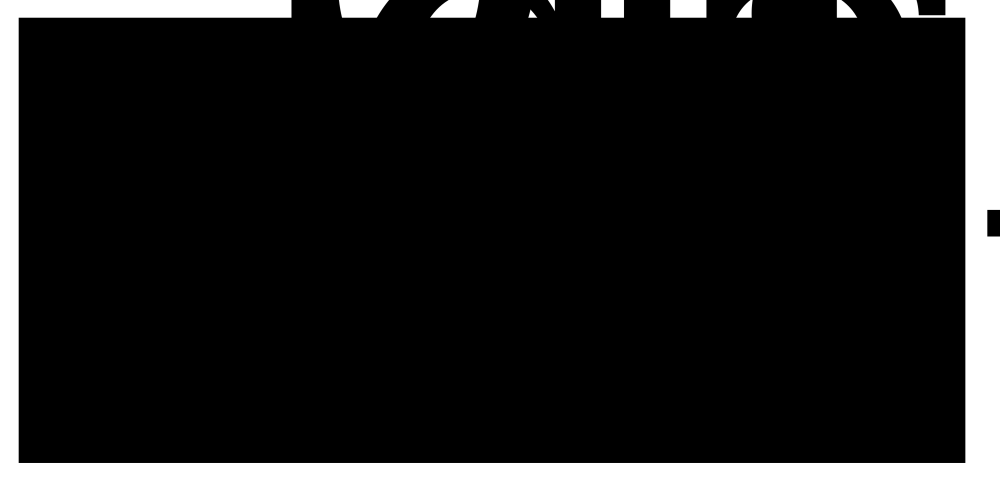
\includegraphics[width=\textwidth]{images/simplified_single_diode_model_simple}
   \caption{ Simplified single diode model for a solar cell }
   \label{fig:simple_EQu_cell}
   \end{center}
   \end{figure}

The maximum-power operating point defines the condition at which the power output (P\textsubscript{\textit{max}} = I\textsubscript{\textit{max}}V\textsubscript{\textit{max}}) of the device is maximal.
The so-called \ac{F.F} is often used to characterize the maximum power ,

\begin{equation}
 \begin{aligned}
  \ac{F.F} = \dfrac{I\textsubscript{\textit{max}}V\textsubscript{\textit{max}}}{I\textsubscript{\textit{sc}}V\textsubscript{\textit{oc}}}
   \label{eq:equ_current_new}
   \end{aligned}
   \end{equation}



\subsection{Double diode model}\label{DDM}
 \begin{figure}[H]
  \begin{center}
  \includegraphics[width=\textwidth]{images/Double_diode_model}
  \caption{ Double diode model for a solar cell }
  \label{fig:Double_EQu_cell}
  \end{center}
  \end{figure}
  
  \begin{equation}
   \begin{aligned}
    I = I\textsubscript{ph} - I\textsubscript{dark} - I\textsubscript{shunt} = I\textsubscript{ph} -  I\textsubscript{s1} (e^{\frac{eV}{\textit{mk}T}}-1) - I\textsubscript{s2} (e^{\frac{eV}{\textit{mk}T}}-1)- \dfrac{V+IR\textsubscript{series}}{R\textsubscript{shunt}}
     \label{eq:equ_current_double}
     \end{aligned}
     \end{equation}
  
\subsection{Equivalent DSCs model}



**Pictures and text about losses in the light absorption in the cell **

**talk ABOUT STABILITY OF dcs with change in temperature **

\section{Maximum power Point Tracking(MPPT)}

**some points form the Introduction can be moved here like the methods of MPP control Algo etc ** \\

Despite all the advantages presented by the generation of energy through the use of PVs, the efficiency of energy conversion is currently low and the initial cost for its implementation is still considered high, and thus it becomes necessary to use techniques to extract the maximum power from these panels, in order to achieve maximum efficiency in operation. It should be noted that there is only one maximum power point (MPP), and this varies according to climatic and irradiation conditions\cite{eltawil2013mppt}.

To overcome this problem, several methods for extracting the maximum power have been proposed in literature **citations **

\subsection{Perturb and Observe Method }
  The \ac{PnO} Method is most widely used in \ac{MPPT} because of  its simple structure and it requires only few parameters. Figure ~\ref{fig:PnOflow}  shows the flow chart of \ac{PnO} method. It perturbs the PV array's terminal voltage periodically, and then it compares the PV output power with that of the previous cycle of perturbation. When PV power and PV voltage increase at the same time and vice versa, a perturbation step size, ${\Delta}$D will be added to the duty cycle, D to generate the next cycle of   perturbation in order to force the operating point moving towards the \ac{MPP}. When PV power increases and PV voltage decreases and vice versa, the perturbation step will be subtracted for the next cycle of perturbation.This process will be carried on continuously until \ac{MPP} is reached.However, the system will oscillate around the \ac{MPP} throughout this process, and this will result in loss of energy. These oscillations can be minimized by reducing the perturbation step size but it slows down the \ac{MPP} tracking system \cite{ngan2011study}.  \\
  
  \begin{figure}[H]
    \begin{center}
    \includegraphics[width=\textwidth]{images/pacehold}
    \caption{ Flow chart for the Perturb and Observe Method }
    \label{fig:PnOflow}
    \end{center}
    \end{figure}
  
  \subsection{Incremental Conductance Method }
  The  solar array terminal  voltage  can  be  adjusted relative to the MPP voltage by measuring the incremental and instantaneous  array  conductance (dI/dV and I/V ,   respectively).  Although  the  incremental  conductance method offers good performance under rapidly changing atmospheric  conditions,  four  sensors  are  required to   perform the  computations. The  drawback is that sensor devices require  more  conversion  time  thus  result in a large amount of power loss.   \\
  
   \begin{figure}[H]
      \begin{center}
      \includegraphics[width=\textwidth]{images/pacehold}
      \caption{ Flow chart for the Incremental Conductance Method}
      \label{fig:inCflow}
      \end{center}
      \end{figure}
  \subsection{fractional open circuit voltage Method }
  This is a method based on the linear relationship between output voltage of the PV array at the \ac{MPP}, V\textsubscript{MPP} and the PV array's open circuit voltage, V\textsubscript{OC} in under varying temperature and solar irradiance. \\
  
  \begin{equation}
    \begin{aligned}
  V\textsubscript{MPP}\approx k\textsubscript{i}V\textsubscript{OC}
  \label{eq:equ_fracoc}
  \end{aligned}
  \end{equation}
  
  Constant value of k\textsubscript{i} is dependent on the characteristics of PV array. Generally, it has to be computed empirically in order to determine the V\textsubscript{MPP} and V\textsubscript{OC} for varied temperatures and solar irradiances. The value of k\textsubscript{i} ranges from 0.73 to 0.80  for most PV modules over a temperature range of 0 to 60$^\circ$C.Figure ~\ref{fig:focflow} describes the operation of a \ac{FOCV}, the PV array is temporarily isolated from \ac{MPPT},then the open circuit voltage, V\textsubscript{OC} is measured periodically by shutting down the power converter momentarily. The \ac{MPPT} calculates V\textsubscript{MPP} from the pre-set value of k1 and the calculated value of V\textsubscript{OC}. Then, the array's voltage is varied until V\textsubscript{MPP} is  reached . The shut-down of power converter periodically will incur temporary loss of power which results in power extracted will not be the maxima. Since is an approximation, the PV array will never reach the \ac{MPP}. Even though this technique is very easy and cheap for implementation, yet since true \ac{MPP} is never reached there is always a loss in power during operation\cite{ngan2011study}.
  
  \begin{figure}[H]
        \begin{center}
        \includegraphics[width=\textwidth]{images/pacehold}
        \caption{ Flow chart for the fractional open circuit voltage Method  Method }
        \label{fig:focflow}
        \end{center}
        \end{figure}
  
\subsection{other Algorithms}
  \begin{itemize}
  \item {\bf Fixed duty cycle} The fixed duty cycle represents the simplest of the methods and it does not require any feedback, where the load impedance is adjusted only once for the maximum power point and it is not adjusted again.
  \item {\bf Pilot cell} In the pilot cell MPPT algorithm, the constant voltage or current method is used, but the open-circuit voltage or short-circuit current measurements are made on a small solar cell, called a pilot cell, that has the same characteristics as the cells in the larger solar array The pilot cell measurements can be used by the MPPT to operate the main solar array at its MPP, eliminating the loss of PV power during the V\textsubscript{OC} or I\textsubscript{sc} measurement
  \item {\bf Fractional short-circuit current }  under varying atmospheric conditions, I\textsubscript{MPP} is approximately linearly related to the I\textsubscript{SC} of the PV array. \newline
    \begin{equation}
      \begin{aligned}
    I\textsubscript{MPP} \approx k\textsubscript{j}I\textsubscript{SC}
    \label{eq:equ_fracoc}
    \end{aligned}
    \end{equation}
   \item {\bf Fuzzy logic controller} (FLC) have the advantages of working with imprecise inputs, it does not need an accurate mathematical model and it can handle non-linearity as well.
  \end{itemize} 
  

\ifx
% Commeted out.

\subsection{**text**\cite{ngan2011study}}

Ngan, Mei Shan, and Chee Wei Tan. "\textit{A study of maximum power point tracking algorithms for stand-alone photovoltaic systems.}" Applied Power Electronics Colloquium (IAPEC), 2011 IEEE. IEEE, 2011. \\

**Text about the paper **

\subsection{**text**\cite{ngan2011study}}

Ngan, Mei Shan, and Chee Wei Tan. "\textit{A study of maximum power point tracking algorithms for stand-alone photovoltaic systems.}" Applied Power Electronics Colloquium (IAPEC), 2011 IEEE. IEEE, 2011. \\

**Text about the paper **

\subsection{**text**\cite{esram2007comparison}}

Esram, Trishan, and Patrick L. Chapman. "\textit{Comparison of photovoltaic array maximum power point tracking techniques.}" IEEE TRANSACTIONS ON ENERGY CONVERSION EC 22.2 (2007): 439.\\

**almost all the Work in eltawil2013mppt is derived from this paper including pictures and text **
\fi


\subsection{**text**\cite{eltawil2013mppt}}

Eltawil, Mohamed A., and Zhengming Zhao. "\textit{MPPT techniques for photovoltaic applications.}" Renewable and Sustainable Energy Reviews 25 (2013): 793-813. \\

This article aims to assess different MPPT techniques, provide background knowledge, implementation topology, grid interconnection of PV and solar microinverter requirements presented in the literature, doing in depth comparisons between them with a brief discussion. The MPPT merits, demerits and classification, which can be used as a reference for future research related to optimizing the solar power generation, are also discussed.\\

**Text about the paper **

\subsection{**text**\cite{reza2013classification}}

Reza Reisi, Ali, Mohammad Hassan Moradi, and Shahriar Jamasb. "\textit{Classification and comparison of maximum power point tracking techniques for photovoltaic system: A review.}" Renewable and Sustainable Energy Reviews 19 (2013): 433-443.

\subsection{**text**\cite{faranda2008energy}}

Faranda, Roberto, and Sonia Leva. "\textit{Energy comparison of MPPT techniques for PV Systems.}" WSEAS transactions on power systems 3.6 (2008): 446-455.\\

This paper presents a comparative study of ten widely-adopted MPPT algorithms; their performance is evaluated on the energy point of view, by using the simulation tool Simulink{\textregistered}, considering different solar irradiance variations.\\

My thesis borrows some of the algorithms/Flow Chart mentioned in the above four papers. 

\subsection{**text**\cite{houssamo2013experimental}}

Houssamo, Issam, Fabrice Locment, and Manuela Sechilariu. "\textit{Experimental analysis of impact of MPPT methods on energy efficiency for photovoltaic power systems.}" International Journal of Electrical Power \& Energy Systems 46 (2013): 98-107.\\

This work presents an experimental comparison; Using four identical PV, under strictly the same set of technical and meteorological conditions, an experimental comparison  of four most used MPPT methods for PV power systems is done.This comparison shows the advantage of use of a MPPT with a variable tracking step.\\  

\subsection{**text**\cite{jain2004new}}
Jain, Sachin, and Vivek Agarwal. "\textit{A new algorithm for rapid tracking of approximate maximum power point in photovoltaic systems.}" Power Electronics Letters, IEEE 2.1 (2004): 16-19.\\

This paper presents a new algorithm for tracking maximum power point in photovoltaic systems. This is a fast tracking algorithm, where an initial approximation of \ac{MPP} quickly achieved using a variable step-size. Subsequently, the exact\ac{MPP} can be targeted using any conventional method like the hill-climbing or incremental conductance method. Thus, the drawback of a fixed small step-size over the entire tracking range is removed, resulting in reduced number of iterations and much faster tracking compared to conventional methods. \\

My implementation draws inspiration for the above article for its  two-stage algorithm to reduce the number of iterations but deviates significantly in the implementation and algorithms used to identify the \ac{MPP} 

\subsection{**text**\cite{liu2011fast}}

Liu, Yi-Hua, and Jia-Wei Huang. "\textit{A fast and low cost analog maximum power point tracking method for low power photovoltaic systems.}" Solar Energy 85.11 (2011): 2771-2780.\\

**add TEXT important RESEARCH * \\

Typically, MPPT methods utilized in medium and high power PV systems uses measured cell characteristics (current, voltage, power) along with an online search algorithm to compute the corresponding \ac{MPP}. Due to the complexity of the required mathematical operations, a \ac{DSP} or a relatively powerful micro-controller is typically needed, which increases the cost of the system.Moreover, it consumes significant portion of the generated power. Therefore, a\ac{MPPT} circuit with low-cost and fast-tracking features is essential .\\

It has already established that there exists a relation between V\textsubscript{MPP} and V\textsubscript{OC} in equation ~\ref{eq:equ_fracoc} and is famously used in the \ac{FOCV} method. However we see that this does not hold true for all illumination conditions and certainly not for low-light(less than ~1500 Lux ) as compared to higher insolation. Since V\textsubscript{OC} is is a logarithmic function of I\textsubscript{ph}, the relationship between  V\textsubscript{MP} and I\textsubscript{MP}.with respect to irradiation is not linear. However, it is possible to linearize this relationship for an interval where the value of V\textsubscript{OC} is sufficiently insensitive to irradiation. That is, the  \ac{VAL} can be calculated as the tangent line of the \ac{MPP} locus where the sensitivity of V\textsubscript{OC} to I\textsubscript{ph} is lower than a pre-defined threshold. This relationship is illustrated in Figure ~\ref{fig:Lui_IV_1} on page ~\pageref{fig:Lui_IV_1}.


 \begin{figure}[H]
  \begin{center}
  \includegraphics[width=\textwidth]{images/IVCurve_lui}
  \caption{I–V curves of the solar panel under different irradiation levels and the voltage approximation line. \cite{liu2011fast} }
  \label{fig:Lui_IV_1}
  \end{center}
  \end{figure}
  
  The same trend can be seen on the I-V curves for the \ac{DSCs} under test (Figure ~\ref{fig:vmmp_lux50_5000}).
   \begin{figure}[H]
    \begin{center}
    \includegraphics[width=\textwidth]{images/IV_50-500}
    \caption{Variation of V\textsubscript{MPP} for different illumination observed **in/on** the DSC under test }
    \label{fig:vmmp_lux50_5000}
    \end{center}
    \end{figure}
  

 \begin{figure}[H]
  \begin{center}
  \includegraphics[width=\textwidth]{images/IVCurve_lui_2}
  \caption{Research Cell Efficiency Records \cite{liu2011fast} }
  \label{fig:Lui_IV_2}
  \end{center}
  \end{figure}





**insert pictures**

\subsection{**text**\cite{dondi2008modeling}}

Dondi, Denis, et al. "\textit{Modeling and optimization of a solar energy harvester system for self-powered wireless sensor networks.}" Industrial Electronics, IEEE Transactions on 55.7 (2008): 2759-2766.\\


**Initial modelling strategies where based on this paper,  improving the efficiency. \# discrete components\# ** 

\subsection{**text**\cite{chu2009robust}}
Chu, Chen-Chi, and Chieh-Li Chen. "\textit{Robust maximum power point tracking method for photovoltaic cells: A sliding mode control approach.}" Solar Energy 83.8 (2009): 1370-1378.\\

\subsection{**text**\cite{urayai2011single}}
Urayai, Caston, and G. Amaratunga. "\textit{Single sensor boost converter-based maximum power point tracking algorithms.}" Applied Power Electronics Conference and Exposition (APEC), 2011 Twenty-Sixth Annual IEEE. IEEE, 2011.\\

Two new maximum power point tracking algorithms are presented: the input voltage sensor, and duty ratio maximum power point tracking algorithm (ViSD algorithm); and the output voltage sensor, and duty ratio maximum power point tracking algorithm (VoSD algorithm).unlike the incremental conductance algorithm which requires two sensors (the voltage sensor and current sensor), the two algorithms are more desirable because they require only one sensor: the voltage sensor.  \\ 

\subsection{**text**\cite{clark2006power}}

Clark, C., and A. Lopez. "\textit{Power system challenges for small satellite missions.}" Proceedings of the 2006 Small Satellites, Systems and Services Symposium, D. Danesy, Ed. The Netherlands: ESA. 2006.\\


**TExt**
Inspiration for use of multiple power buses 



\section{Machine Learning ???}
This section discusses about Search optimization in order to lock on the  V\textsubscript{MP} and I\textsubscript{MP} as efficiently as possible.

\subsection{Regression Modelling \cite{lenarreg2006}}

We use regression analysis when we want to predict one variable from another. The most basic form of regression is called simple regression, where We have 1 independent variable and 1 dependent variable and where we are predicting a linear trend. In regression, we attempt to determine the magnitude of the relationship between a set of independent variables and the dependent variable. Independent variable(X), Also called the predictor variable, that we believe influences our Dependent variable(Y),Also called the response variable.\\

A regression model is a formal way of stating:
\begin{itemize}
\item The tendency of the response variable(Y) to vary with the predictor variable(X).
\item A scattering of points around some statistical relationship.
\end {itemize}

Equation for a line can be written as:

\begin{equation}
\begin{aligned}
  y= mx + b 
\label{eq:Line_equ}
\end{aligned}
\end{equation}

The linear regression model(for observation i = 1, . . . , N) can we written as:

\begin{equation}
\begin{aligned}
  Y\textsubscript{i}= \beta\textsubscript{0}+\beta\textsubscript{1}X\textsubscript{i} +\epsilon\textsubscript{i}
\label{eq:Line_equ}
\end{aligned}
\end{equation}

\begin{itemize}
\item $\beta\textsubscript{0}$ is the mean of the population when X is zero -the Y intercept.\\
\item $\beta\textsubscript{1}$ is the slope of the line, the amount of increase in Y brought about by a unit increase $(X^{'}= X + 1)$ in X.\\
\item \textbf{$\epsilon\textsubscript{i}$} is the random error, specific to each observation.
\end {itemize}



**add more text about line Linear Regression **


\subsection{Pattern search}

Seiler, Mary C., and Fritz A. Seiler. "\textit{Numerical recipes in C: the art of scientific computing.- 10.2 Golden Section Search in One dimention}" Risk Analysis 9.3 (1989): 415-416.\\

Finding the Maxima or minima of a first order single variable function can easily be found by equating the derivative of this function to zero. However finding the derivative of certain functions is not always easy or possible.In such conditions Search techniques are used to find the Maxima or minima in a uni-modal((A uni-modal function contains only one minimum or maximum on the specified interval ) continuous function over an interval without using derivatives.  Golden Section search Algorithm is one such search method. The Algorithm derives its name from the Golden ratio(0.61803...)\\

Two numbers are said to be in the golden ratio if their ratio is same as the ratio of their sum to the larger of the two quantities.Assuming b > a then this can be expressed as:\\

\begin{equation}
\begin{aligned}
 \dfrac{a+b}{b}=\dfrac{b}{a}=\phi
\label{eq:golden_ratio1}
\end{aligned}
\end{equation}

where ${\phi}$ is the golden ratio whose value is given by:\\

\begin{equation}
\begin{aligned}
 \phi=\dfrac{\sqrt{5}-1}{2}= 0.61803398874989......
\label{eq:golden_ratio}
\end{aligned}
\end{equation}
**add more text about Golden search **
\begin{figure}[H]
  \begin{center}
  \includegraphics[width=\textwidth]{images/pacehold}
  \caption{ Golden Section search Algorithm }
  \label{fig:Golden_search}
  \end{center}
  \end{figure}